\documentclass[a4paper,11pt]{article}
\usepackage[utf8]{inputenc}
\usepackage{minted}
\usepackage{amsmath}
\usepackage{float}
\usepackage[symbol]{footmisc}
\usepackage{graphicx}
\usepackage{multirow}
\usepackage{array}
\usepackage[toc,page]{appendix}

\graphicspath{{./figures/}}
\renewcommand{\thefootnote}{\fnsymbol{footnote}}

\title{\textbf{10. Hash table}}
\author{Kristiāns Vinters}
\date{Fall 2023}

\begin{document}
    \maketitle
    \section*{Introduction}

    I solved the assignment in Go. I used Go because I want to become more familiar with it. Source code and benchmark data is available on GitHub\footnote[1]{https://github.com/Phanty133/id1021/tree/master/10-hashmap}.

    \section*{Implementation}

    There weren't any particular difficulties in implementing a hash table (hash map) in Go for use with the \texttt{postnummer} dataset.

    The hashmap was defined with a simple struct.

    \begin{minted}{go}
type NodeHashMap struct {
    buckets    [][]Node
    numBuckets int
}
    \end{minted}

    The hash map is created by the \texttt{CreateHashMap()} function, which takes the parsed CSV data and number of buckets as arguments.

    \begin{minted}{go}
func CreateHashMap(data []Node, numBuckets int) *NodeHashMap {
    hashMap := NodeHashMap{
        buckets:    make([][]Node, numBuckets),
        numBuckets: numBuckets,
    }

    for _, node := range data {
        hash := node.CodeNum % numBuckets

        if hashMap.buckets[hash] == nil {
            hashMap.buckets[hash] = make([]Node, 0)
        }

        hashMap.buckets[hash] = append(hashMap.buckets[hash], node)
    }

    return &hashMap
}
    \end{minted}

    The lookup function takes a zip code as a string and returns a pointer to the node with the given zip code and the number of elements in the bucket, which is used for benchmarking. The function first calculates the hash, then finds the right entry in the resulting bucket. If the entry is not found, \texttt{nil} is returned.

    \begin{minted}{go}
func (data *NodeHashMap) Lookup(zip string) (*Node, int) {
    zipNum, err := ZipToNum(zip)
    // ... Error handling here ...

    hash := zipNum % data.numBuckets

    for _, node := range data.buckets[hash] {
        if node.Code == zip {
            return &node, len(data.buckets[hash])
        }
    }

    return nil, 0
}
    \end{minted}

    \section*{Benchmarking}

    I performed benchmarks for \texttt{111 15} and \texttt{984 99} lookup for all implementations,as well as hash map lookup time vs bucket count and number of collisions on the \texttt{postnummer} dataset vs bucket count. All measurements were repeated 5000 times.

    For analyzing run times, I measured the raw execution time for every repeat in nanoseconds, which I stored in an array and then wrote to a \texttt{.csv} file. I used LibreOffice Calc to calculate the mean, median, min, and max times and plot the graphs.

    \section*{Implementation comparison}

    Fig. \ref{fig:lookups} shows the lookup times for the various implementations. For \texttt{111 15} all implementations are very fast, but for \texttt{984 99} the linear search is by far the slowest. The reason is because the linear search starts from index 0, which happens to be \texttt{111 15}, whereas \texttt{984 99} is on the other end of the dataset. Because of the small dataset, it's difficult to distinguish between the runtimes of the other algorithms. Overall, the fastest median time is for the integer binary search, but that's because the plain map and hash maps take a string parameter, so there's a conversion overhead. If the plain map and hash map were to take an integer parameter, they would be as fast as the binary search.

    \begin{figure}[H]
        \centering
        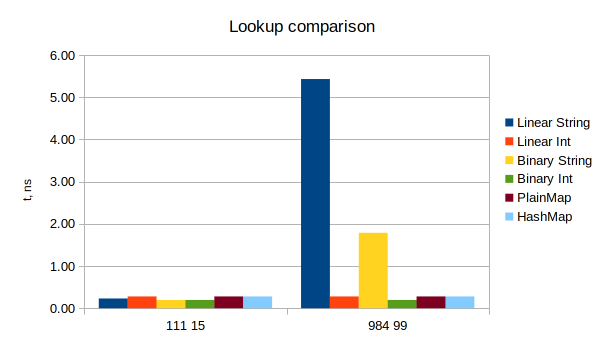
\includegraphics[width=\textwidth]{lookups.png}
        \caption{Lookup times for the various implementations.}
        \label{fig:lookups}
    \end{figure}

    \begin{figure}[H]
        \centering
        
        \begin{tabular}{c|c|c|c}
            \textbf{Value} & \textbf{Type} & \textbf{Algorithm} & \textbf{Median time, ns} \\
            \hline
            \hline
            \multirow{6}{*}{\texttt{111 15}} & \multirow{4}{*}{String} & Linear search & 0.23 \\
            & & Binary search & 0.28 \\
            & & Plain map & 0.28 \\
            & & Hash map & 0.28 \\
            \cline{2-4}
            & \multirow{2}{*}{Integer} & Linear search & 0.20 \\
            & & Binary search & 0.20 \\
            \hline
            \multirow{6}{*}{\texttt{984 99}} & \multirow{4}{*}{String} & Linear search & 5.43 \\
            & & Binary search & 0.28 \\
            & & Plain map & 0.28 \\
            & & Hash map & 0.28 \\
            \cline{2-4}
            & \multirow{2}{*}{Integer} & Linear search & 1.79 \\
            & & Binary search & 0.20 \\
        \end{tabular}

        \caption{Implementation lookup median times}
        \label{fig:lookup-table}
    \end{figure}

    When comparing string and integer lookups, integer lookups are noticeably faster. The difference isn't as great for binary search ($0.08ns$), but for linear search there's a $3.0x$ performance improvement. This is because integer comparisons are significantly faster than string comparisons. When comparing strings, you need to compare each character, whereas integers can be compared in a single operation. The reason why there's a lesser improvement for binary search is because the linear search performs significantly more comparisons.

    \section*{Bucket collisions}

    I measured the number of collisions in the \texttt{postnummer} dataset for every modulo from 1 to 100000 and plotted in fig. \ref{fig:collisions}. The relationship is non-linear, with the number of collisions decreasing exponentially as the modulo increases.

    \begin{figure}[H]
        \centering
        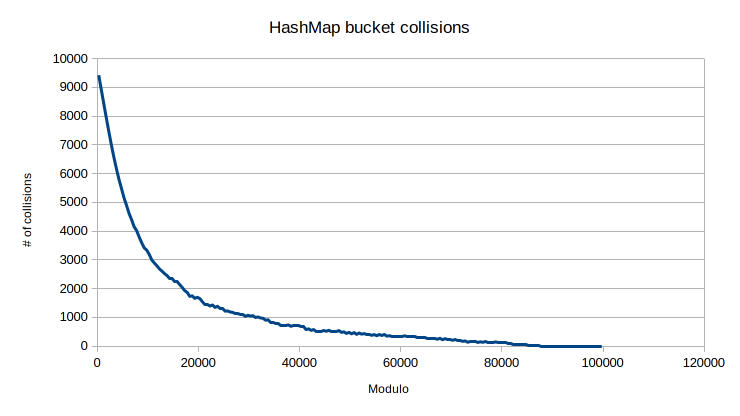
\includegraphics[width=\textwidth]{collisions.png}
        \caption{Bucket collisions vs modulo}
        \label{fig:collisions}
    \end{figure}

    \section*{Hash map lookup time vs bucket count}

    I benchmarked 5000 random, consistent lookups for hash map modulo 10, 100, 500, 1000, 2500, 5000, 7500, 10000, 15000, 25000, 37500, 50000, 62500, 75000, 100000. The results are shown in fig. \ref{fig:hashmap}. The lookup time increases as the modulo decreases, therefore mean bucket size increases. While the bucket size keeps decreasing after modulo 100, the lookup time doesn't decrease as much. Therefore, an optimal modulo for this particular dataset appears to be between 100 and 1000.

    \begin{figure}[H]
        \centering
        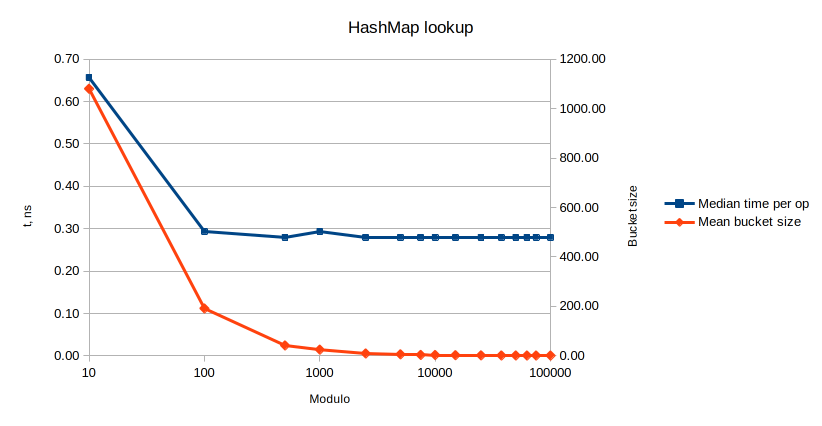
\includegraphics[width=\textwidth]{hashmap.png}
        \caption{Hash map median lookup time and mean bucket size. Left Y axis is lookup time, right Y axis is bucket size.}
        \label{fig:hashmap}
    \end{figure}
\end{document}
